% !Mode:: "TeX:UTF-8"
%% udesoftec-doc.tex
%% Copyright 2015 J. Peter M. Schuler
%% 2021/02/22 v1.7.1 udesoftec
\documentclass[de,omit-sd,omit-lol]{udesoftec} 
\usepackage{udesoftec-extra}

\usetikzlibrary{shadows}
\newcommand*\keystroke[1]{%from http://tex.stackexchange.com/questions/5226/keyboard-font-for-latex
  \tikz[baseline=(key.base)]
    \node[%
      draw,
      fill=white,
      drop shadow={shadow xshift=0.15ex,shadow yshift=-0.15ex,fill=black,opacity=0.75},
      rectangle,
      rounded corners=1pt,
      inner sep=.5pt,
      line width=0.5pt,
      font=\scriptsize\sffamily
    ](key){\strut{}#1};%
}

\newcommand{\BibTeX}{BibTeX}
    

\typeofdoc{Dokumentation zu}
\title{udesoftec}
\subtitle{\LaTeX{}-Formatvorlage  \linebreak für Qualifikationsarbeiten am  \linebreak Lehrstuhl für  \linebreak Wirtschaftsinformatik und Softwaretechnik}
\author{J. Peter M. Schuler}
\entitle{[\hyperref[sec:abstract]{English summary available}]}
\city{Essen}
\labelPreTopic{}
\institution{Universität Duisburg-Essen}
\semester{}                       
\authorbox{
\begin{tabularx}{.7\linewidth}{ll}
  Maintainer:&J. Peter M. Schuler\\
        &j.peter.m.schuler@uni-due.de\\
    \\
\end{tabularx}
}
\date{\udesoftecversion}

\abstract{
This LaTeX package provides a documentclass for use in written theses at the
University of Duisburg-Essen, Research Group for Business Informatics and
Software Engineering. It is based on pdflatex and bibtex using KOMA-Script and
natbib and  many other popular packages. The current documentation is only
available in german. However the  \hyperref[sec:classoptions]{class options in
section \ref*{sec:classoptions}} and \hyperref[sec:variables]{configuration
variables for the titlepage in section \ref*{sec:variables}} should be quite
understandable and the paket list in the \hyperref[sec:classinstall]{tlmgr
command} shows where to
look for further information. A \hyperref[sec:exampleproject]{MWE and a download
of an example project is also available in section \ref*{sec:exampleproject}.} 

If you just intend to use the BibTeX style without the documentclass simply
using package udesoftec-bst should be sufficient.
If you just intend to use the BibLaTeX style without the documentclass simply
using package udesoftec-biblatex should be sufficient.} 
\abstractEn{ Install with MikTeX or if using TeX Live (e.g. BasicTeX) with
\lstinline!tlmgr! using the command mentioned in section \ref{sec:classinstall}.

    An alternative, in case you run into problems: just install the documentclass and bibstyle from ctan. Afterwards 
    download the appropiate cover from \url{http://mirror.ctan.org/macros/latex/contrib/udesoftec} and place it next to 
    your document's \lstinline!main.tex!.}


\renewcommand{\udesoftecoverride}{
    \renewcaptionname{ngerman}{\labelabstracttitle}{English summary for this document}
    %\renewcaptionname{english}{\labelabstracttitle}{Installation}
    \renewcaptionname{british}{\labelabstracttitle}{Installation}
}                   
%%%%%%%%%%%%%%%%%%%%%%%% DOCUMENT %%%%%%%%%%%%%%%%%%%%%%%%
\begin{document}    
\newacronym[description={User Interface, \entode{Benutzeroberfläche}}]{ui}{UI}{User Interface}
\newacronym[description={Business-to-Customer, \entode{Unternehmen-zu-Kunde}, beschreibt den Zielmarkt für Transaktionen}]{b2c}{B2C}{Business-to-Customer}
\newglossaryentry{Pattern}{name=Pattern, description={TODO:Pattern Definition}}
\newglossaryentry{Pattern-Kategorie}{name=Pattern-Kategorie, description={Die Einteilung eines \gls{Pattern} in einem Pattern-Katalog}}

\chapter{Einführung}

\section{Grundidee}
Dieses Template stellt eine professionelle Lösung für die Nutzung von \LaTeX{} bereit, die an einigen Stellen von den Quick'and'Dirty und den Plattformübergreifenden Lösungen aus gutem Grund abweicht. Dementsprechend wird über das Template hinaus eine eher spezifische Konfiguration der \LaTeX{}-Umgebung empfohlen. Ein paar Beispiele dafür:

\begin{itemize}
    \item es werden direkt und ausschließlich PDF-Dokumente generiert und kein DVI oder PS als Ergebnis.
    \item durchgehende UTF-8-Nutzung (trotz \LaTeX{} statt XeLaTeX)
    \item eingebettete Grafiken liegen ausschließlich im PDF-Format vor
\end{itemize}

\section{Beispiel-Projekt}\label{sec:exampleproject}
Ein funktionierendes Dokument lässt sich durch folgendes Beispiel (MWE - minimum working example) erstellen:
\begin{lstlistinglatex}[label=lst:mwe,caption=Minimal Working Example für udesoftec]
\documentclass{udesoftec}
\begin{document}
Inhalt
\end{document}
\end{lstlistinglatex}
Grundsätzlich sind kaum Einstellungen und Konfigurationen notwendig. Lediglich Dinge wie der Inhalt und die bib-Datenbank sind einzufügen.
Ein Beispielprojekt mit echten Inhalten findet sich unter\newline \url{http://udue.de/udesoftecexample}


%%%%%%%%%%%%%%%%%%%%%%%%%%%%%%%%%%%%%%%%%%
\pagebreak% looks nicer 
\section{Klassenparameter und Konstanten}
%%%%%%%%%%%%%%%%%%%%%%%%%%%%%%%%%%%%%%%%%%
\subsection{Optionen der Klasse}\label{sec:classoptions}
\begin{description}[leftmargin=2.75cm,style=sameline] 
    \item[biber]{Benutzung von BibLaTeX und biber statt BibTeX}
    \item[proposal]{Bspw. für ein Exposé. Setzt alle omit-* Optionen.}
    \item[final]{Deaktiviert einige Funktionen (bspw. TODOs) und beschleunigt einige Ausgaben.}
    \item[en]{Wechselt die primäre Dokumentsprache von Deutsch auf Englisch. Ändert einzelne Überschriften und andere sprachabhängige Labels.}
    \item[printlayout]{Wechselt auf doppelseitiges Druck-Layout ("`Buchlayout"') und Serien-Schrift. Nützlich, wenn die Arbeit ausgedruckt wird und beidseitiger Druck möglich ist. Kapitel beginnen auf rechten Seiten, dadurch werden Leerseiten eingefügt.}
    \item[confidential]{Erstellt einen Sperrvermerk, vgl. \autoref{sec:sperrvermerk}.}
    \item[long-a]{Für deutsche Dokumente: Wenn die beiden Abstracts so lang sind, dass sie nicht auf eine Seite passen, fängt der englische auf einer neuen Seite an.}
    \item[omit-a]{Abstract entfernen.}
    \item[omit-lot]{Tabellenverzeichnis entfernen.}
    \item[omit-lof]{Abbildungsverzeichnis entfernen.}
    \item[omit-loa]{Abkürzungsverzeichnis entfernen.}
    \item[omit-sd]{Eidesstattliche Versicherung entfernen.}
    \item[omit-toc]{Inhaltsverzeichnis entfernen.}
    \item[omit-todos]{TODO-Liste am Ende des Dokuments entfernen.}
    \item[vawiessen]{Passt das Deckblatt an die Vorgaben von VAWi-Essen an.}
    \item[vawibamberg]{Passt das Deckblatt an die Vorgaben von VAWi-Bamberg an.}
\end{description}

\pagebreak% looks nicer 
\subsection{Anpassen des Deckblatts}\label{sec:variables}
Neben den Paket-Optionen \lstinlinelatex!vawiessen! und \lstinlinelatex!vawibamberg! können die folgenden Kommandos vor dem \lstinlinelatex!\begin{document}! genutzt werden:

\begin{multicols}{4}
    \begin{itemize}
        \item \lstinlinelatex!\typeofdoc!
        \item \lstinlinelatex!\academicfield!
        \item \lstinlinelatex!\authorbox!
        \item \lstinlinelatex!\institution!
        \item \lstinlinelatex!\semester!
        \item \lstinlinelatex!\entitle!
        \item \lstinlinelatex!\city!
        \item \lstinlinelatex!\confidSource!
    \end{itemize}
\end{multicols}
             
            
Darüber hinaus gibt es natürlich noch die Standard-Kommandos:
\begin{multicols}{3}
    \begin{itemize}
        \item \lstinlinelatex!\title!
        \item \lstinlinelatex!\author!
        \item \lstinlinelatex!\date!
    \end{itemize}
\end{multicols}
Die Nutzung ist wie bei den Standard-LaTeX-Kommandos üblich:
\begin{lstlistinglatex}[label=lst:configuration,caption=Beispiel für Konfigurations-Commandos für das Deckblatt]
\title{Meine Bachelorarbeit}
\entitle{My Bachelor Thesis}
\author{Max Musterman}
\authorbox{
    \begin{tabularx}{.7\linewidth}{ll}
        von:        &Max Mustermann\\
                    &Musterstrasse 123\\
                    &12345 Musterstadt\\
        \\
        Gutacher:   &Prof. Dr. Stefan Eicker\\
                    &Prof. Dr. John Doe\\
        \\
        Betreuer:   &Dipl.-Wirt.-Inf Some Body\\
        \\
    \end{tabularx}  
}\end{lstlistinglatex}

\subsection{Sperrvermerke}\label{sec:sperrvermerk}
Durch die Klassenoption \lstinlinelatex!confidential! wird der Sperrvermerk aktiviert und durch die Neudefinition des Firmennamens über den Befehl \lstinlinelatex!\confidSource!, kann Sie entsprechend angepasst werden:
\begin{lstlistinglatex}[label=lst-confidentialitySource,caption=Sperrvermerke aktivieren]
    \documentclass[confidential]{udesoftec}
    \confidSource{Name der Firma}
\end{lstlistinglatex}




\chapter{Nutzung der Formatvorlage und übliche Kommandos}


\section{Beispiele für Zitationen}

Die häufigsten Zitationsarten sind hier vermerkt, eine komplette Liste der Möglichkeiten findet sich bspw. im \href{http://merkel.zoneo.net/Latex/natbib.php}{Natbib Cheat Sheet}

\subsection{Wörtliche Zitate eines Absatzes mit Quellenangabe}

Zitate als Absätze machen vor allem bei vollständigen Aussagen oder umfangreichen Definitionen Sinn:
\citequotepar[xix]{Tidwell.2011}{The text that started it all dealt with physical buildings, not software. Christopher Alexander’s A Pattern Language and its companion book The Timeless Way of Building established the concept of patterns and described a 250-pattern multilayered pattern language.}
\begin{lstlistinglatex}[label=lst:citequotepar,caption=Wörtliche Zitate eines vollständigen Absatzes mit Quellenangabe]
\citequotepar[<Seite>]{<Quelle>}{<Text>}
\end{lstlistinglatex}

\subsection{Wörtliche Zitate im Fließtext mit Quellenangabe}

Wörtliche Zitate im Fließtext machen vor allem bei kleineren Auszügen Sinn:
\parExample[Wörtliche Zitate im Fließtext mit Quellenangabe]{Die meisten Autoren sehen als Ausgangspunkt die Architektur: \citequote[xix]{Tidwell.2011}{The text that started it all dealt with physical buildings [\ldots]}}
\begin{lstlistinglatex}[label=lst:citequote,caption=Wörtliche Zitate im Fließtext mit Quellenangabe]
\citequote[<Seite>]{<Quelle>}{<Text>}
\end{lstlistinglatex}


\subsection{Quellenangaben im Fließtext}
Für Quellenangaben im Fließtext wird folgende Variante genutzt:
\parExample[nicht-wörtliches Zitat]{Merkmale von Patterns sind u.a.
Abstraktionsgrad, Domänenbezug und Sprache \cite[541]{Fettke.et.al.2009}.} \begin{lstlistinglatex}[label=lst:cite,caption=Quellenangaben im Fließtext]
\cite[<Seite>]{<Quelle>}
\end{lstlistinglatex}


\subsection{Autorennamen im Text mit Quellenangabe}
Wenn der Autorenname im Text erwähnt wird, sollte dieser immer direkt auch die Jahresangabe (oder sogar Seitenzahl) für das Werk enthalten, da man in der Regel nicht wirklich den Autor erwähnt, sondern Aussagen oder Forschungsergebnisse der Person zu einem bestimmten Zeitpunkt. Theoretisch könnte man zuerst nur den Namen erwähnen und am Ende des Gedankenganges dann die Quelle, es ist aber zielführender die Quellenangabe und Autorenangabe nicht zu trennen:
\parExample[Autorennamen im Text mit Quellenangabe]{Systemakzeptanz ist nach \citet[24]{Nielsen.1993} die grundlegende Frage dahingehend, [...]. }
\begin{lstlistinglatex}[label=lst:citet,caption={Autorennamen im Text mit Quellenangabe}]
\citet[<Seite>]{<Quelle>}
\end{lstlistinglatex}
\parExample[Autorennamen im Text ohne Quellenangabe]{Dabei unterteilt \citeauthor{Nielsen.1993} diese Akzeptanz in verschiedene Bereiche.}
\begin{lstlistinglatex}[label=lst:citeauthor,caption={Autorennamen im Text ohne Quellenangabe}]
\citeauthor{<Quelle>}
\end{lstlistinglatex}%

\subsection{Mehrere Werke in Quellenangaben}
Manchmal wird ein Gedanke durch mehrere unterschiedliche Quellen gestützt. Hier kann man folgendes Verfahren nutzen und bspw. als \lstinline!<prefix>! ein "`vgl. z.\ B."' nutzen:
\parExample[mehrere Werke in Quellenangabe]{Dementsprechend wird für die
Usability mit dem Fokus auf das Web, in der Literatur entsprechend der Begriff
der Web Usability verwendet \citemulti{vgl. z.~B. \cite[146]{Matera.2006};
\cite[xix]{Nielsen.et.al.2006}; \cite[11]{Schweibenz.et.al.2003}}.}
\begin{lstlistinglatex}[label=lst:citemulti,caption={Mehrere Werke in
Quellenangaben}] 
\citemulti{<prefix>\cite[<Seite>]{<Quelle>};\cite[<Seite2>]{<Quelle2>}...}
\end{lstlistinglatex}

\subsection{Quellenangabe für Normen und Standards (bspw. ISO, DIN)}
Da Normen immer äußerst schwierig in Citavi und BibTeX sind, gibt es einen
neuen Dokumenttyp \lstinline!@techstandard!. Die vollständige Norm-Nummer sollte im BibTeX-Feld \lstinline!standard! ausgegeben
werden. Alternativ wird aus \lstinline!type!,\lstinline!number! und
\lstinline!edition! eine Nummer gebildet.
\begin{lstlistingbibtex}[label=lst:normbib,caption={Angabe einer Norm im
BiB-File}]
@techstandard{IEEEStd-1016:1998,
 year = {1998-09-23},
 title = {IEEE Recommended Practice for Software Design Descriptions},
 edition = {1998},
 number = {1016},
 author = {IEEE},
 type = {IEEE Std},
 standard = {IEEE Std 1016-1998}
}
\end{lstlistingbibtex}
Dies kann man im Rahmen des BibTeX-Exports von Citavi einstellen:
\begin{itemize}
    \item Den Titel in Citavi anlegen:\begin{enumerate}
    \item Dokumententyp: Norm
\item Institution: IEEE
\item Titel:IEEE Recommended Practice for Software Design Descriptions
\item Normtyp:IEEE Std
\item Nummer:1016
\item Ausgabedatum:1998-09-23
\item Freitext 1: IEEE Std 1016-1998
 \end{enumerate}
    \item Dann den Export aufrufen: Menu Datei => Exportieren => Exportieren...
    \item Alle Titel und Weiter
    \item BibTeX und Bearbeiten
    \item bei Dokumenttyp zuordnen \enquote{Norm} dem Typ \enquote{techstandard}
    zuordnen und Weiter
    \item Für Dokumenttyp "Norm"; Feld "Freitext 1" als Wert "standard"
    eintragen
\end{itemize}
Aufgrund dessen, dass in der
vollständigen Norm-Nummer allerdings schon das Jahr enthalten ist, wird dieses
nicht im Fließtext zusätzlich ausgegeben. Daher muss für eine Ausgabe analog zu 
\textbf{Autorennamen im Text mit Quellenangabe} statt \lstinlinelatex!\citet{}!
ein \lstinlinelatex!\citeauthor{}! mit anschließender Seitenangabe genutzt.
\parExample[Quellenangabe für Normen und Standards (bspw. ISO, DIN)]{Diese
Verfahren sind näher in \citeauthor{IEEEStd-1016:1998} \citetext{S. 16}
geregelt.} \begin{lstlistinglatex}[label=lst:citestd,caption={Quellenangabe für Normen und Standard}]
\citeauthor{IEEEStd-1016:1998} \citetext{S. 16}
\end{lstlistinglatex}


\section{Abbildungen}

Abbildungen werden ausschließlich als PDF eingefügt. Dadurch sind Sie einfacher wartbar und die Chance, dass beim Erstellen eine Vektorgrafik produziert wird steigt gegenüber anderen Vorgehensweisen. Jedes Programm kann grundsätzlich PDF exportieren (selbst MS Powerpoint) und ein PDF-Drucker wie \href{http://www.dopdf.com/de/}{doPDF} versorgt die restlichen Programme. 

Im Gegensatz zur anderen Textprogrammen ist folgendes wichtig zu wissen: Die Position der Abbildung bestimmt LaTeX, nicht der Autor. Daher sollten Abbildungen so im Text genutzt werden, dass es egal ist, ob Sie an der geplanten Stelle, auf der selben Seite darüber, oder erst einzelne Seiten später plaziert wird.
\parExample[Abbildungen einfügen]{Dabei unterteilt \citeauthor{Nielsen.1993} die Akzeptanz in verschiedene Bereiche (vgl. \autoref{fig:Nielsen_1993_Acceptability}).}
%%%%%%%%%%%%%%%%%%% FIGURE %%%%%%%%%%%%%%%%%%%%%%
\begin{figure}
    \centering{
            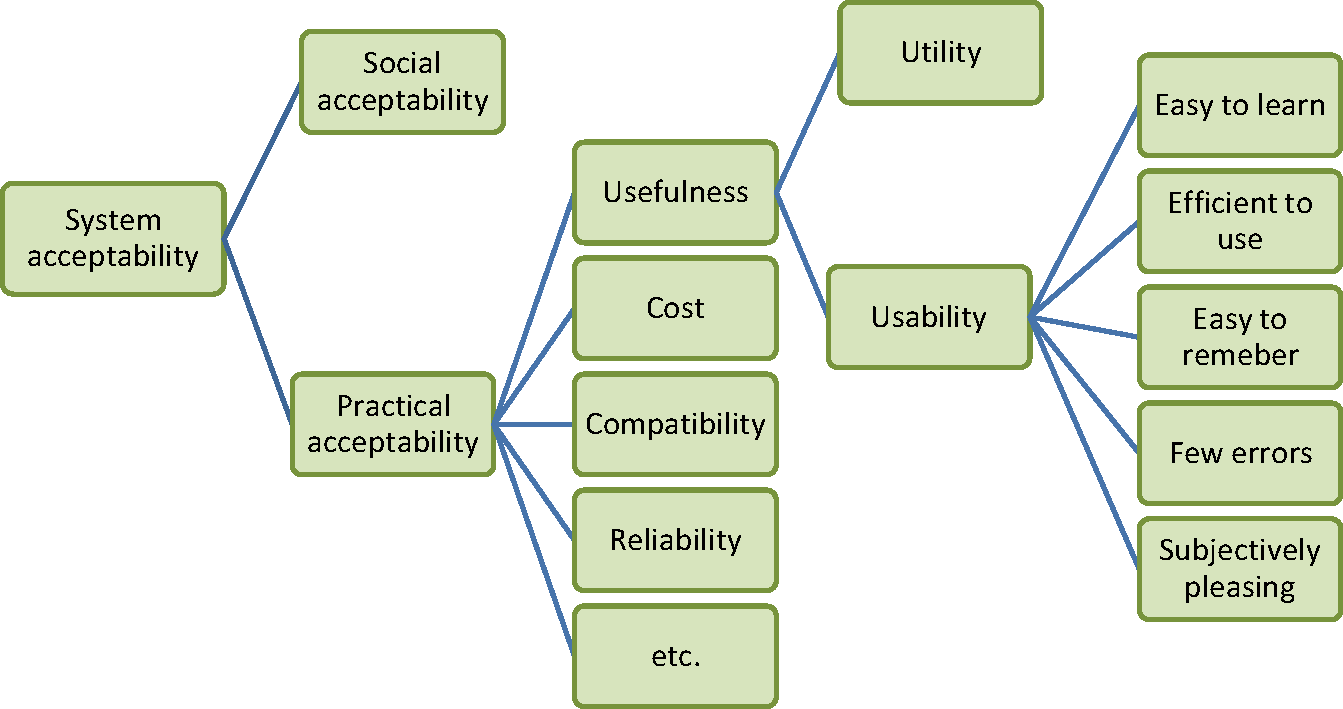
\includegraphics[width=.95\linewidth,keepaspectratio=true]{udesoftec-doc-exampleimage}
            \caption[System Akzeptanz nach \citeauthor{Nielsen.1993}]{System Akzeptanz nach \citet[25]{Nielsen.1993}}%
            \label{fig:Nielsen_1993_Acceptability}%
        }%
\end{figure}%
%%%%%%%%%%%%%%%%%%% FIGURE %%%%%%%%%%%%%%%%%%%%%%


\begin{lstlistinglatex}[label=lst:figure,caption={Abbildungen einfügen}]
Dabei unterteilt \citeauthor{Nielsen.1993} die Akzeptanz in verschiedene Bereiche (vgl. \autoref{fig:Nielsen_1993_Acceptability}).
%%%%%%%%%%%%%%%%%%% FIGURE %%%%%%%%%%%%%%%%%%%%%%
\begin{figure}
    \centering{
        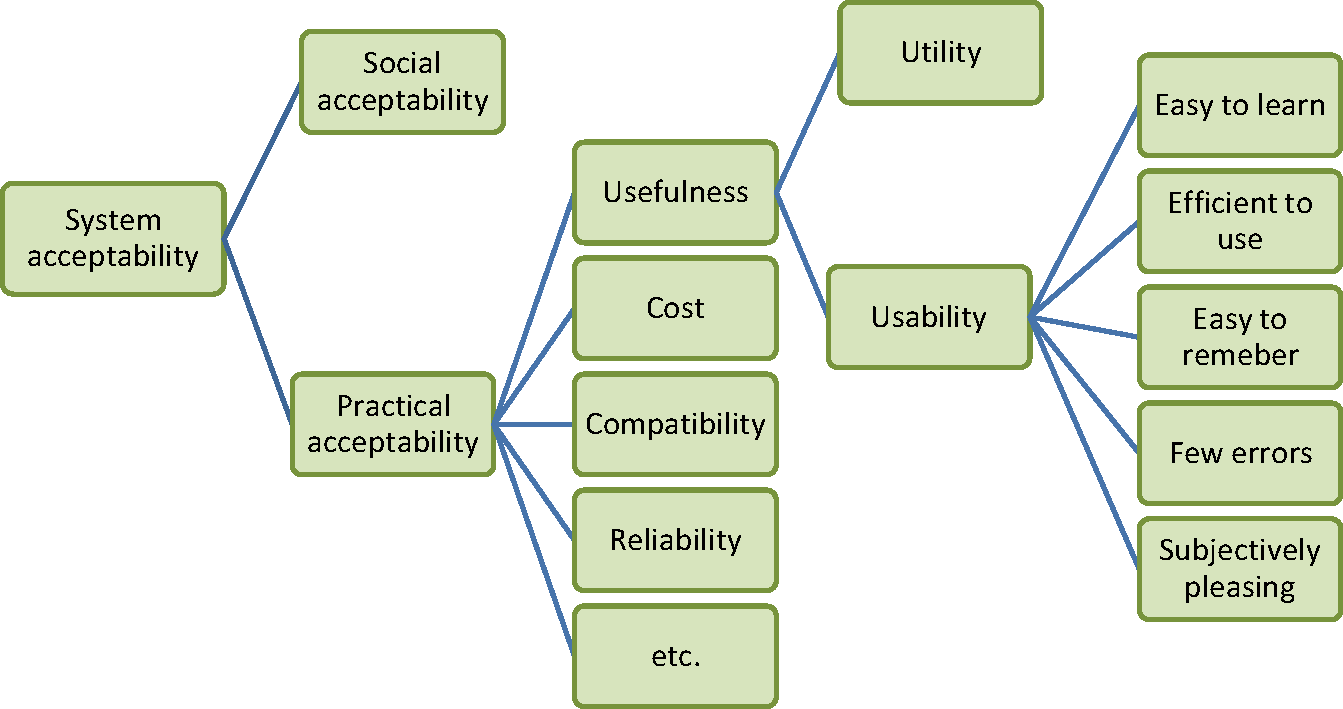
\includegraphics[width=.95\linewidth,keepaspectratio=true]{udesoftec-doc-exampleimage}
        \caption[System Akzeptanz nach \citeauthor{Nielsen.1993}]{System Akzeptanz nach \citet[25]{Nielsen.1993}}%
        \label{fig:Nielsen_1993_Acceptability}%
    }%
\end{figure}%
%%%%%%%%%%%%%%%%%%% FIGURE %%%%%%%%%%%%%%%%%%%%%%
\end{lstlistinglatex}




\section{Abkürzungen}
Über das folgende Kommando können Abkürzungen angelegt werden:
\begin{lstlisting}[language={[LaTeX]TeX},morekeywords={\newacronym}]
\newacronym[<Erlaeuterung>]{<intern>}{<Abkuerzung>}{<Ausgeschrieben>}
\end{lstlisting}
Als Wert für \lstinline!<intern>! hat sich die Kleinschreibung der Abkürzung bewährt, also bspw.:
\begin{lstlisting}[language={[LaTeX]TeX},morekeywords={\newacronym}]
\newacronym{din}{DIN}{Deutsches Institut für Normung}
\end{lstlisting}
Über die folgenden Kommandos können Abkürzungen genutzt werden, wobei \lstinline!\acr! bei erster Verwendung ausschreibt:
\begin{lstlisting}[language={[LaTeX]TeX},morekeywords={\acr,\acrshort}]
\acr{<intern>} oder \acrshort{<intern>}
\end{lstlisting}
Bspw.: Abkürzungen wie \acr{b2c} können eingeführt und danach kurz als \acr{b2c} genutzt werden, oder wie bei \acrshort{ui} trotz erstmaliger Verwendung kurzgeschrieben werden.



\section{Aufzählungen}
\subsection{Aufzählungslisten unnummeriert}
Beschreibungslisten können auch mit festem Einschub gesetzt werden:
\parExample[Aufzählungslisten unummeriert]{
\begin{itemize}
    \item{Lorem ipsum dolor sit amet, consetetur sadipscing elitr, sed diam nonumy eirmod tempor invidunt ut labore et dolore magna aliquyam erat, sed diam voluptua.}
    \item{Stet clita kasd gubergren, no sea takimata sanctus est Lorem ipsum dolor sit amet.}
\end{itemize}
}
\begin{lstlistinglatex}[label=lst:itemize,caption={Aufzählungslisten unummeriert}]
\begin{itemize}[leftmargin=3.5cm]
    \item{Lorem ipsum dolor...}
    \item{Stet clita kasd...}
\end{itemize}
\end{lstlistinglatex}

\subsection{Aufzählungslisten nummeriert}
Nummerierte Aufzählungslisten sind auch möglich.
\parExample[Aufzählungslisten nummeriert]{
\begin{enumerate}
    \item{Lorem ipsum dolor sit amet, consetetur sadipscing elitr, sed diam nonumy eirmod tempor invidunt ut labore et dolore magna aliquyam erat, sed diam voluptua.}
    \item{Stet clita kasd gubergren, no sea takimata sanctus est Lorem ipsum dolor sit amet.}
\end{enumerate}}
\begin{lstlistinglatex}[label=lst:enumerate,caption={Aufzählungslisten nummeriert}]
\begin{enumerate}
    \item{Lorem ipsum dolor...}
    \item{Stet clita kasd...}
\end{enumerate}
\end{lstlistinglatex}
Für eine Anpassung der Form (beispielsweise aufzählen mit Buchstaben, Text vor den Zahlen etc.) sei auf die \lstinline!\label!-Option verwiesen, die bspw. unter \url{http://de.wikibooks.org/wiki/LaTeX-Wörterbuch:_enumitem} erklärt ists.

\subsection{Merkmal-Aufzählungen mit festem Einschub}
Beschreibungslisten können auch mit festem Einschub gesetzt werden:
\parExample[Merkmal-Aufzählungen mit festem Einschub]{
\begin{description}[leftmargin=2.5cm,style=sameline]
    \item[Merkmal]{Lorem ipsum dolor sit amet, consetetur sadipscing elitr, sed diam nonumy eirmod tempor invidunt ut labore et dolore magna aliquyam erat, sed diam voluptua.}
    \item[Element]{Stet clita kasd gubergren, no sea takimata sanctus est Lorem ipsum dolor sit amet.}
\end{description}}
\begin{lstlistinglatex}[label=lst:desc-sameline,caption={Merkmal-Aufzählungen mit festem Einschub}]
\begin{description}[leftmargin=2.5cm,style=sameline]
    \item[Merkmal]{Lorem ipsum dolor...}
    \item[Element]{Stet clita kasd...}
\end{description}
\end{lstlistinglatex}

\subsection{Merkmal-Aufzählungen mit Umbruch}
Beschreibungslisten können auch mit festem Umbruch gesetzt werden:
\parExample[Merkmal-Aufzählungen mit Umbruch]{
\begin{description}[style=nextline]
    \item[Merkmal]{Lorem ipsum dolor sit amet, consetetur sadipscing elitr, sed diam nonumy eirmod tempor invidunt ut labore et dolore magna aliquyam erat, sed diam voluptua.}
    \item[Element]{Stet clita kasd gubergren, no sea takimata sanctus est Lorem ipsum dolor sit amet.}
\end{description}}
\begin{lstlistinglatex}[label=lst:desc-nextline,caption={Merkmal-Aufzählungen mit Umbruch}]
\begin{description}[style=nextline]
    \item[Merkmal]{Lorem ipsum dolor...}
    \item[Element]{Stet clita kasd...}
\end{description}
\end{lstlistinglatex}

\section{TODOs}
Über \lstinlinelatex!\todo{<Text>}! und \lstinlinelatex!\inlinetodo{<Text>}! gibt es die Möglichkeit TODOs zu verwalten. \inlinetodo{TODO: Diese können innerhalb des Textes stehen wie hier.} Aber Sie können auch am Rand  stehen und auf eine bestimmte Stelle im Text\todo{TODO: Absatz überarbeiten} zeigen. Am Ende des Dokuments wird eine Gesamtliste angefügt, sofern ein TODO existitert und das Dokument nicht mit der Option \lstinlinelatex!final! oder \lstinlinelatex!omit-todos! kompiliert wird.



\chapter{FAQ}

\section{Warning: Biber: there were undefined citations}
Ist aktuell ein known issue, allerdings kann kein Fehler in der Ausgabe festgestellt werden.

\section{BibTeX Fehler: Paragraph ended before \ldots parsedate was complete.}
Irgendwo gibt es in der .bib-Datei ein Fehlerhaftes Datum (urldate). Das Datum
sollte im Format dd.mm.yyyy oder yyyy-mm-dd vorliegen (oder weder \enquote{.}
noch \enquote{-} im String haben).

\section{Der Hinweis mit der Template-Version auf dem Deckblatt soll verschwinden}
Vor der Abgabe sollte mit dem Kommando \lstinlinelatex!\date{}! das Datum des Dokuments entfernt werden. Dadurch wird auch der Hinweis auf die Templateversion entfernt. Während der Bearbeitung können beide Hinweise aber beim Feedback hilfreich sein.

\section{Bei kursiver Schrift ist das "`a"' komisch}
Das ist korrekt. Bei kursiver Schrift wird bspw. in MS Word oftmals einfach der normale Font schräg gestellt. In professionellen Systemen werden extra \emph{Schriftschnitte} erstellt. Die in dieser Vorlage benutzte Schriftart ist \sfdefault{} (screenlayout) sowie \rmdefault{} (printlayout). Hierbei existiert ein solcher Schriftschnitt. Da das kleine "`a"' in "`schräg"' aber sehr merkwürdig aussehen würden, sind Sie leicht anders entworfen. Bei anderen Schriften kann dies bspw. auch das \&-Zeichen betreffen.
\parExample[unterschiedliche Schriftschnitte]{
\begin{tabularx}{\linewidth}{ll}
Screenlayout normal:& \textsf{Schriften \& anderes}\\
Screenlayout kursiv:& \textsf{\emph{Schriften \& anderes}}\\
Printlayout normal:& \textrm{Schriften \& anderes}\\
Printlayout kursiv:& \textrm{\emph{Schriften \& anderes}}\\
\end{tabularx}  
}

\section{Im Literaturverzeichnis steht manchmal "`Auflage"' statt "`Aufl."'}
Das \BibTeX-Feld Auflage (bzw. Edition) sollte als Wert in aller Regel nur eine Zahl enthalten, bspw. "`3"'. Dann erstellt der Zitierstil je nach Sprache automatisch ein "`3. Aufl."' oder "`3\textsuperscript{rd} edn."'. In seltenen Fällen kann es sein, dass eine Zahl nicht korrekt ist (bspw. "`Reprint 2008"'). Sollte der Zitierstil keine Zahl finden, wird einfach der gesamte Inhalte des Feldes genutzt. Folglich wäre "`Aufl."' das richtige Verhalten und wenn stattdessen "`Auflage"' steht, sollte der \BibTeX{}- bzw. Citavi-Eintrag angepasst werden.

\section{LaTeX Error: File `udesoftec-cover-ude-de' not found.}
Anscheinend kann die \TeX{}-Distribution die Cover-Dateien nicht finden. Das lässt auf eine veraltete Version der Klasse schließen. In diesem Fall (nach einem Update der packages)einfach das passende Cover von der \href{http://mirror.ctan.org/macros/latex/contrib/udesoftec}{Paket-Seite auf CTAN} heruntergeladen und in den selben Ordner wie die Hauptdatei des Projektes (z.B. \lstinline!main.tex!) gelegt werden.

\section{Das Abkürzungsverzeichnis erscheint nicht}

Es gab ein Problem in v1.4.4, das seit v1.4.5 behoben ist. Zusätzlich kann es sein, dass die makeindex-Befehle nicht ausgeführt werden, z. B.:

\lstinline!makeindex -s file.ist -t file.alg -o file.acr file.acn!

Wie genau dieser Befehl aussieht, ist von der TeX-Umgebung abhängig.

\section{Das Abkürzungsverzeichnis ist doppelt}

vgl. \autoref{sec:updateinstructions}

\section{LaTeX Error: Error: Undefied control sequence - Package enumitem Error: undefined.}

vgl. \autoref{sec:updateinstructions}

\section{LaTeX Error: Error: Undefied control sequence - Package enumitem Error:1,5cm unde-
fined.}

vgl. \autoref{sec:updateinstructions}
\section{LaTeX Error: File '****.sty' not found.}
Wahrscheinlich wird in einer neueren Version der Klasse ein zusätzliches Paket genutzt, das noch nicht installiert ist. Das sollte vor allem nicht-MikTeX-(Windows)-Konfigurationen betreffen. Hierfür einfach das aktualisierte Kommando unter 
vgl. \autoref{sec:classinstall} nutzen.
%%%%%%%%%%%%%%%%%%%%%%%% APPENDIX %%%%%%%%%%%%%%%%%%%%%%%
\appendix% \addcontentsline{toc}{chapter}{Anhang}




\def\chapterAuthor{ }
\chapter{Anhang}
\section{Installation und Konfiguration der Software}\label{sec:software}
Grundsätzlich wird immer empfohlen Updates für die Software-Pakete einzuspielen. Sollte sich die Ausgabe verändern, bspw. weil udesoftec neue Features erhält, finden Sie in \autoref{sec:updateinstructions} und im \hyperref[sec:changelog]{ChangeLog} entsprechende Hinweise wie das Dokument anzupassen ist.

\subsection{LaTeX-Umgebung: MikTeX (Windows), BasicTeX (OSX)}\label{sec:classinstall}
Unter Windows wird ausdrücklich \href{http://miktex.org}{MikTeX} empfohlen, da dieses selbständig und On-Demand fehlende Dinge nachinstalliert. 

Unter MacOS kann beispielsweise ein minimales \TeX{}-Live-System wie
\href{http://tug.org/mactex/morepackages.html}{BasicTeX} genutzt werden. Die
notwendigen Pakete lassen sich wie folgt installieren (mehrere tlmgr install
Kommandos für einfacheres Copy-and-Paste):
\begin{lstlisting}[label=lst:tlmgr,caption={Paket-Installation der Documentclass und ihrer Abhängigkeiten},language=bash,breaklines=true,morekeywords={sudo},emph={tlmgr,install,update,--self,--all},
        keywordstyle=\color{DocumentDark4},
        emphstyle=\color{DocumentDark1}]
sudo tlmgr update --self
sudo tlmgr update --all
sudo tlmgr install udesoftec nag chngcntr hyphenat libertine mweights fontaxes footmisc placeins 
sudo tlmgr install enumitem todonotes wallpaper marginnote mdframed needspace csquotes glossaries 
sudo tlmgr install glossaries-german glossaries-english xfor datatool substr xstring tracklang biblatex 
sudo tlmgr install logreq regexpatch datetime2 datetime2-german datetime2-english mfirstuc
\end{lstlisting} 

\subsection{Citavi}
Citavi erlaubt nur noch manuelle \BibTeX-Exporte, die \href{http://support.citavi.de/forum/viewtopic.php?f=156&t=7295&p=24152}{Funktion für automatischen Export ist entfernt worden}. Der Export funktioniert einfach über das Datei Menü (\href{http://www.citavi.com/sub/manual4/de/exporting_to_bibtex.html}{Anleitung zum \BibTeX-Export in der Citavi-Hilfe}).
        
\subsection{Editor für TeX-Dokumente}
Es gibt viele Editoren für TeX-Dokumente, hilfreich ist die sogenannte "SyncTeX"-Unterstützung, mit der man über einen Klick zwischen Quellcode und Ausgabeposition hin und herspringen kann.

\subsubsection{Visual Studio Code}
Der kostenloase \href{https://code.visualstudio.com/download}{Visual Studio Code} mit dem Plugin \href{https://marketplace.visualstudio.com/items?itemName=James-Yu.latex-workshop}{LaTeX Workshop} scheint eine komfortable Alternative zu sein.

\subsubsection{ShareLaTeX} 

\href{https://www.sharelatex.com}{www.sharelatex.com} ist ein SaaS-Anbieter. Kaum etwas zu konfigurieren, dafür teilweise ältere Versionen.
\section{Update Instructions}\label{sec:updateinstructions}
This documentclass is as downwards compatible as possible. Any change in the version number according the third digit (e.g. from 1.2.1 to 1.2.8) creates no compile or display errors.
Some changes however cannot be catched, so that in case of major version changes some LaTeX errors and warnings may occure. The following list shows some changes to the document one should do in order to remove the errors and warnings.

\subsection{Update to 1.5.0}
\begin{enumerate}
  \item You might get compile errors with broken urldate in bib files.
  \item You might get compile errors if you have conditional language
  statements or use other packages as language switched from ``english'' to
  ``british''
\end{enumerate}

\subsection{Update to 1.4.0}
Removed many packages and removed some deprecated commands. Might raise problems with custom loaded packages or if e.g. \ctanlink{verbatim}-commands were used instead of \ctanlink{lstlisting}-commands.

\subsection{Update to 1.3.8}
Added abstract as default, so fill values \lstinlinelatex!\abstract! and perhabs \lstinlinelatex!\abstractEn!.

\subsection{Update to 1.3.0}
\begin{description}[style=nextline]
  \item[Change in document configuration sets main page to default values]{All configuration labels like \lstinlinelatex!\def \institution{Name}! are not working anymore and need to be replaced with real commands like \lstinlinelatex!\institution{Name}!. }
    \item[Error: Undefied control sequence - Package enumitem]{Happens while using \lstinlinelatex!\begin{description}[\breaklabel]!. \newline{} Due to a new package the option is now \lstinlinelatex!style=nextline!, so use\newline{} \lstinlinelatex!\begin{description}[style=nextline]! instead.

Happens while using \lstinlinelatex!\begin{description}[\setleftmargin{1.5cm}]]!.\newline{} Due to a new package the option is now \lstinlinelatex!leftmargin=1.5cm!, so use\newline{} \lstinlinelatex!\begin{description}[leftmargin=1.5cm,style=sameline]! instead.
}
    
\end{description}
\subsection{Update to 1.2.1}
\lstinlinelatex!\printacronyms! not necessary any more - the documentclass takes care of this.


\clearpage\section{Changelog}\label{sec:changelog}
An \href{http://pipes.yahoo.com/jpmschuler/udesoftec?_render=rss}{RSS feed} is available to annouce new versions of udesoftec.
\begingroup
    \lstinputlisting[backgroundcolor={},frame=none,nolol,breaklines=true]{CHANGELOG.txt}
\endgroup
\bibliography{udesoftec-doc-examplebib} % output Literature and use this file as bibtext catalogue
\end{document}